%%%%%%%%%%%%%%%%%%%%%%%%%%%%% Define Article %%%%%%%%%%%%%%%%%%%%%%%%%%%%%%%%%%
\documentclass{article}
%%%%%%%%%%%%%%%%%%%%%%%%%%%%%%%%%%%%%%%%%%%%%%%%%%%%%%%%%%%%%%%%%%%%%%%%%%%%%%%

%%%%%%%%%%%%%%%%%%%%%%%%%%%%% Using Packages %%%%%%%%%%%%%%%%%%%%%%%%%%%%%%%%%%
\usepackage[margin = 1 in]{geometry}
\usepackage{graphicx}
\usepackage{amssymb}
\usepackage{amsmath}
\usepackage{amsthm}
\usepackage{empheq}
\usepackage{mdframed}
\usepackage{booktabs}
\usepackage{lipsum}
\usepackage{graphicx}
\usepackage{color}
\usepackage{psfrag}
\usepackage{pgfplots}
\usepackage{bm}
%%%%%%%%%%%%%%%%%%%%%%%%%%%%%%%%%%%%%%%%%%%%%%%%%%%%%%%%%%%%%%%%%%%%%%%%%%%%%%%

% Other Settings

\usepackage[spanish]{babel}
\usepackage{hyperref}
\hypersetup{
    colorlinks=true,
    linkcolor=blue,
    urlcolor=red,
    pdftitle={How to write a thesis},
    }
\usepackage{fancyvrb}
\usepackage{fancyhdr, lastpage}
\pagestyle{fancy}
\lhead{Universidad Autónoma de Nuevo León}
\rhead{Facultad de Ingeniería Mecánica y Eléctrica}
\cfoot{Page \thepage\ of \pageref{LastPage}}
%%%%%%%%%%%%%%%%%%%%%%%%%% Page Setting %%%%%%%%%%%%%%%%%%%%%%%%%%%%%%%%%%%%%%%
\geometry{a4paper}

%%%%%%%%%%%%%%%%%%%%%%%%%% Define some useful colors %%%%%%%%%%%%%%%%%%%%%%%%%%
\definecolor{ocre}{RGB}{243,102,25}
\definecolor{mygray}{RGB}{243,243,244}
\definecolor{deepGreen}{RGB}{26,111,0}
\definecolor{shallowGreen}{RGB}{235,255,255}
\definecolor{deepBlue}{RGB}{61,124,222}
\definecolor{shallowBlue}{RGB}{235,249,255}
%%%%%%%%%%%%%%%%%%%%%%%%%%%%%%%%%%%%%%%%%%%%%%%%%%%%%%%%%%%%%%%%%%%%%%%%%%%%%%%

%%%%%%%%%%%%%%%%%%%%%%%%%% Define an new command %%%%%%%%%%%%%%%%%%%%%%%%
\newcommand{\setcover}{{\bfseries Set covering }}
\newcommand{\ds}{\displaystyle}
%%%%%%%%%%%%%%%%%%%%%%%%%%%%%%%%%%%%%%%%%%%%%%%%%%%%%%%%%%%%%%%%%%%%%%%%%%%%%%%

%%%%%%%%%%%%%%%%%%%%%%%%%% Define an orangebox command %%%%%%%%%%%%%%%%%%%%%%%%
\newcommand\orangebox[1]{\fcolorbox{ocre}{mygray}{\hspace{1em}#1\hspace{1em}}}
\usepackage[most]{tcolorbox}
%%%%%%%%%%%%%%%%%%%%%%%%%%%%%%%%%%%%%%%%%%%%%%%%%%%%%%%%%%%%%%%%%%%%%%%%%%%%%%%

%%%%%%%%%%%%%%%%%%%%%%%%%%%% English Environments %%%%%%%%%%%%%%%%%%%%%%%%%%%%%
\newtheoremstyle{mytheoremstyle}{3pt}{3pt}{\normalfont}{0cm}{\rmfamily\bfseries}{}{1em}{{\color{black}\thmname{#1}~\thmnumber{#2}}\thmnote{\,--\,#3}}
\newtheoremstyle{myproblemstyle}{3pt}{3pt}{\normalfont}{0cm}{\rmfamily\bfseries}{}{1em}{{\color{black}\thmname{#1}~\thmnumber{#2}}\thmnote{\,--\,#3}}
\theoremstyle{mytheoremstyle}
\newmdtheoremenv[linewidth=1pt,backgroundcolor=shallowGreen,linecolor=deepGreen,leftmargin=0pt,innerleftmargin=20pt,innerrightmargin=20pt,]{theorem}{Theorem}[section]
\theoremstyle{mytheoremstyle}
\newmdtheoremenv[linewidth=1pt,backgroundcolor=shallowBlue,linecolor=deepBlue,leftmargin=0pt,innerleftmargin=20pt,innerrightmargin=20pt,]{definition}{Definition}[section]
\theoremstyle{myproblemstyle}
\newmdtheoremenv[linecolor=black,leftmargin=0pt,innerleftmargin=10pt,innerrightmargin=10pt,]{problem}{Problem}[section]
%%%%%%%%%%%%%%%%%%%%%%%%%%%%%%%%%%%%%%%%%%%%%%%%%%%%%%%%%%%%%%%%%%%%%%%%%%%%%%%

%%%%%%%%%%%%%%%%%%%%%%%%%%%%%%% Plotting Settings %%%%%%%%%%%%%%%%%%%%%%%%%%%%%
\usepgfplotslibrary{colorbrewer}
\pgfplotsset{width=8cm,compat=1.9}
%%%%%%%%%%%%%%%%%%%%%%%%%%%%%%%%%%%%%%%%%%%%%%%%%%%%%%%%%%%%%%%%%%%%%%%%%%%%%%%

%%%%%%%%%%%%%%%%%%%%%%%%%%%%%%% Title & Author %%%%%%%%%%%%%%%%%%%%%%%%%%%%%%%%
\title{Tarea 1: Set Covering}
\author{Lic. Arnoldo Del Toro Peña}
%%%%%%%%%%%%%%%%%%%%%%%%%%%%%%%%%%%%%%%%%%%%%%%%%%%%%%%%%%%%%%%%%%%%%%%%%%%%%%%

\begin{document}
\maketitle
\newpage
Sea el universo $\varTheta $ y la familia  $Z$ de subconjuntos de $\varTheta $, una cobertura es una familia $C \subseteq  Z$ cuya unión es $\varTheta $
\\ El problema de \setcover tiene la siguiente formulación:
\begin{gather}
    \text{Minimizar: } \sum_{S \in Z } p(S) x_S \label{1} \\
    \sum_{S:e \in Z} x_S \geq 1 \hspace{0.3in} \forall e  \in \varTheta \label{2} \\
    x_S \in \{0,1\} \hspace{0.3in} \forall S  \in Z \label{3}
\end{gather}

En la ecuación \ref{2} se trata de cubrir todas los elementos de $\varTheta$ .
\\ En la ecuación \ref{3} se trata para todo conjunto este o no en el conjunto de cobertura.
\\ En la ecuaión \ref{1} se trata de minimizar los costos al seleccionar un subconjunto de cobertura.
\\ Para obtener una solución al problema aplicaremos los siguientes pasos: \vspace{0.1 in}
\begin{tcolorbox}[colback=yellow!50!black,colframe=brown!50!black,title=Pasos a seguir: ]
    \begin{enumerate}
        \item Seleccionaremos el subconjunto  $s$ de menor costo tal que $s \in Z$.
        \item Agregaremos este elemento al conjunto inicialmente vacio $C$.
        \item Si la unión de todos los subconjuntos actualmente seleccionados es igual a $\varTheta $ $\left( \displaystyle \bigcup_{i \in C} {x_i} = \varTheta \right)$ entonces hemos terminado, en caso contrario haremos el paso 4.
        \item Quitaremos el subconjunto seleccionado de $Z$. Después, de los subconjuntos restantes quitaremos los elementos ya cubiertos por el actual $s$; regresar al paso 1.
    \end{enumerate}
\end{tcolorbox}
El diagrama se muestra en la figura \ref{diagrama}.
\begin{figure}[h!]
    \centering
    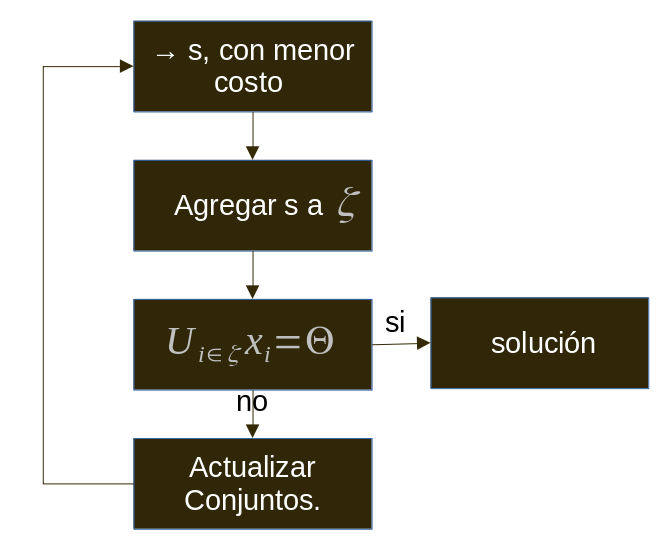
\includegraphics[scale = 0.40]{diagrama set covering.png}
    \caption{Diagrama algoritmo \setcover}
    \label{diagrama}
\end{figure}
\newpage
Veamos el siguiente ejemplo:
\\ Sea $\varTheta = \{ 1,2,3,4,5 \}$  y $Z = \{ A,B,C,D \}$ donde:
$$A= \{ 1,2,3 \}$$
$$B= \{4,5 \}$$
$$C= \{ 1,2,5\}$$
$$D= \{1,3,5 \}$$
Donde $p_i = \{5,3,2,1\}$ con $i \in \{A,B,C,D\}$ son los costos por seleccionar cada subconjunto.
\\ Seleccionaremos el subconjunto con el menor costo:
\[s= D\]
Sea $\zeta  = \{D\}$ \\
Verificaremos que: $\left( \displaystyle \bigcup_{i \in \zeta } {x_i} = \varTheta \right)$,
\[ \ds \{1,3,5\} \neq \varTheta  \] 
Sea: $$Z = \{A,B,C\}$$
\begin{gather*}
    A = \{2\} \\
    B = \{4\} \\
    C = \{2\} 
\end{gather*}

% segunda iteración
Seleccionaremos el subconjunto con el menor costo:
\[s= C\]
Sea $\zeta = \{D,C\}$ \\
Verificaremos que: $\left( \displaystyle \bigcup_{i \in \zeta} {x_i} = \varTheta \right)$,
\[ \ds \{1,2,3,5\} \neq \varTheta  \] 
Sea: $$Z = \{B\}$$
\begin{gather*}
    B = \{4\} 
\end{gather*}
Si observamos $Z$ solamente quedó compuesta de $B$, esto debido a que $A$ quedó vacío.

%tercera iteración
Seleccionaremos el subconjunto con el menor costo:
\[s= B\]
Sea $\zeta = \{D,C,B\}$ \\
Verificaremos que: $\left( \displaystyle \bigcup_{i \in \zeta} {x_i} = \varTheta \right)$,
\[ \ds \{1,2,3,4,5\} = \varTheta  \] 
Hemos terminado, solución: $\zeta = \{D,C,B\}$, con un costo de 6.



\end{document}